\section{Methodology}\label{sec:method}

\begin{figure*}[!t]
    \centering
    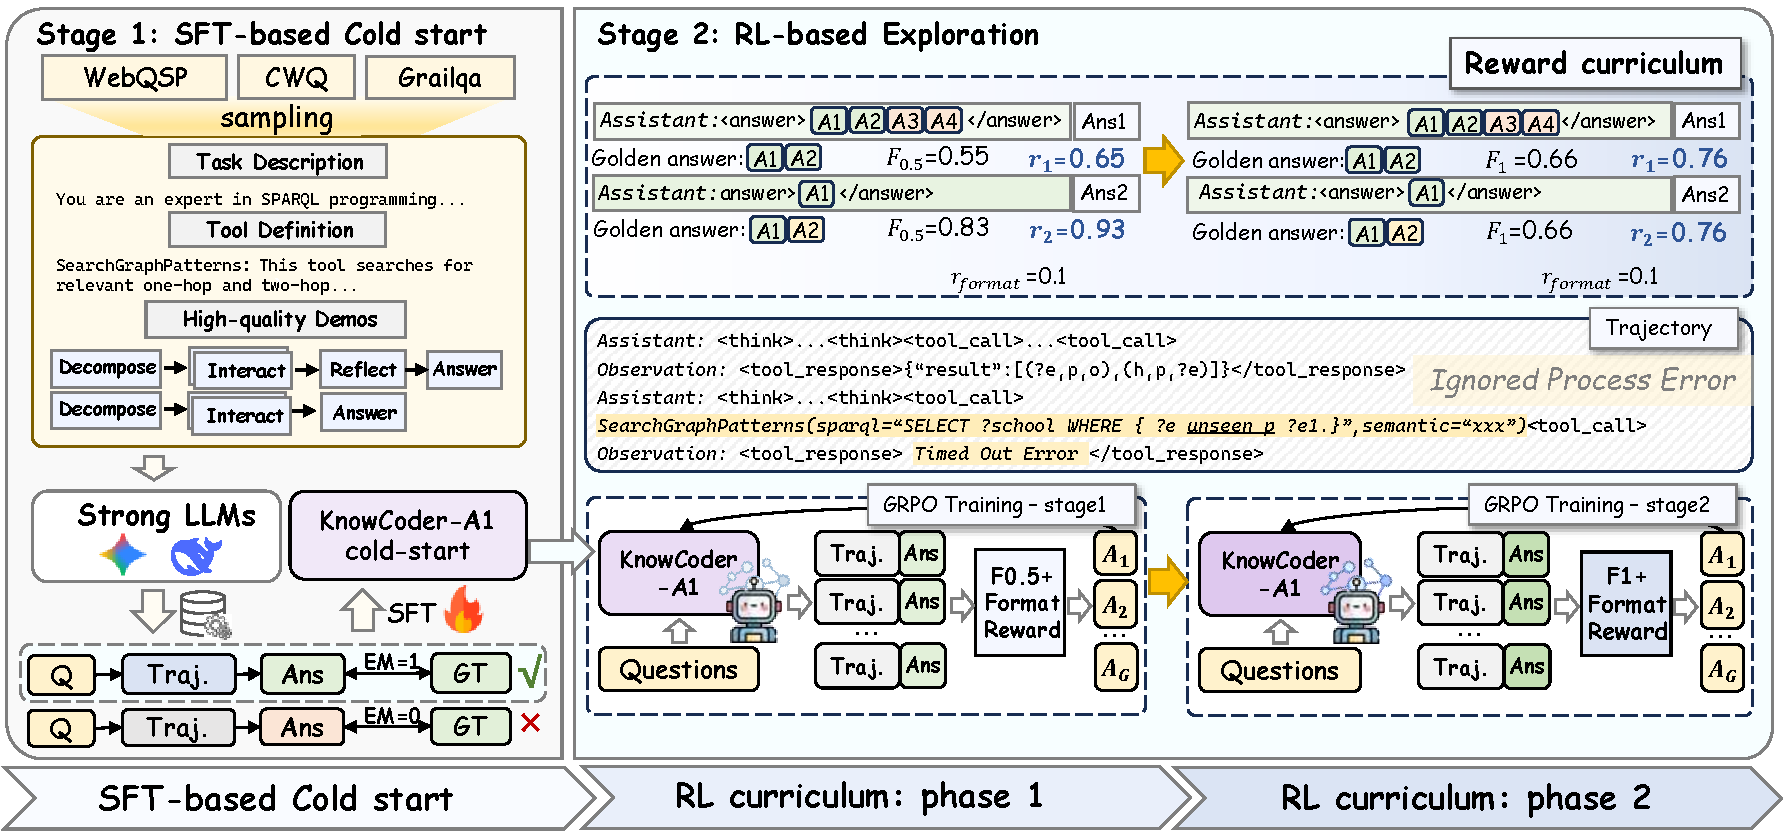
\includegraphics[width=\textwidth]{figures/main.pdf}
    \caption{An overview of the training framework of \ours \space. Stage 1 (left): the SFT-based cold-start process, where high-quality trajectories are curated from strong LLMs to fine-tune an initial agent. Stage 2 (right): the multi-phase Reinforcement Learning curriculum, where the agent is progressively improved through exploration and a dynamic reward strategy.}
    \label{fig:main}
\end{figure*}


\subsection{Agentic Initialization}
\ours \space follows a ReAct-style~\citep{yao2023react} agent paradigm that interleaves explicit reasoning and tool use over a KB environment, and terminates with a final answer.

\textbf{Environment.} We view the KB and the tool executor as the environment:
$\mathcal{M}=(\mathcal{G},\ \texttt{Exec})$,
where \texttt{Exec} executes tool calls against $\mathcal{G}$ and returns structured observations (including error diagnostics when execution fails). It is worth noting that error messages are retained to provide corrective signals to help LLM refine subsequent tool calls.

\textbf{Action Space.} At each step, the agent first produces an explicit thinking process and then makes a tool call from a finite action set $\textsc{Action}$. We instantiate three tools based on Interactive-KBQA~\citep{xiong2024interactive}:
\begin{itemize}
    \item \textsc{SearchTypes}(typename): Given a type name, retrieves and ranks candidate types in similarity order.
    \item \textsc{SearchGraphPatterns}(sparql, semantic): Given a partial SPARQL sketch (assumed to start with \texttt{SELECT DISTINCT ?x WHERE \{...\}}), returns up to 10 one- and two-hop subgraphs in which the variable \texttt{?x} appears as the head or tail object. An optional \texttt{semantic} parameter can be provided to rank the returned subgraphs in similarity order.
    \item \textsc{ExecuteSPARQL}(sparql): Given a SPARQL query, executes it against a sandboxed endpoint over $\mathcal{G}$ and returns the result. This enables flexible query on the graph, such as hypothesis testing (e.g., subgraph existence) or end-to-end query execution.
\end{itemize}

\textbf{State and Trajectory.}
Let $c_t$ denote the explicit thinking process in natural language, $a_t\in \textsc{Action}$ the action, and $o_t$ the observation at step $t$. The trajectory, which also serves as the agent's state, is the history of all past interactions. The trajectory at step $t$ is denoted as:
\begin{equation}
\tau_t = \{(c_1,a_1,o_1),\ldots,(c_{t},a_{t},o_{t})\}.
\end{equation}

\textbf{Interactive Process.}
Given a question $q$, the agent begins with an initial prompt 
\begin{equation}
\mathrm{Prompt}=\big(\mathrm{Inst},\ q,\ E_q\big),
\end{equation}
where the instruction consists of a brief task description, tool definitions, and the required interaction format, followed by the question $q$ and its topic entities $E_q$. The specific prompt is provided in the Appendix~\ref{app:prompt}.

At each step $t$, the agent first generates a thought $c_{t+1}$ and a tool call $a_{t+1}$ conditioned on the current trajectory and the initial prompt:
\begin{equation}
c_{t+1}, a_{t+1} = \mathrm{LLM}(\tau_t, \mathrm{Prompt}).
\end{equation}

The tool call $a_{t+1}$ is then passed to the executor, which returns an observation $o_{t+1} = \texttt{Exec}(a_{t+1})$. The new interaction turn $(c_{t+1}, a_{t+1}, o_{t+1})$ is appended to the current trajectory to form the trajectory for the next step, $\tau_{t+1}$. This iterative process continues until the agent determines it has gathered sufficient information and decides to output the final answer, or reaches $T$, the maximum number of steps.

\subsection{SFT-based Cold-start Stage}
Due to the heterogeneous structures of KBs and the complexity of questions, employing a base model with insufficient reasoning and tool-use capabilities as an agent makes it difficult to guarantee the discovery of trajectories to the correct answer. To mitigate this issue, we introduce a cold-start stage where the agent is fine-tuned on reasoning trajectories to acquire foundational perception and reasoning capabilities. Instead of relying on program-decomposed trajectories, we generate trajectories via outcome-based rejection sampling. Moreover, to avoid overfitting while ensuring sufficient guidance, we adhere to the principle of constructing a dataset that is concise, yet high in quality and diversity. In the following, we will first describe this data curation process and then detail the model's training procedure. 

\subsubsection{Data Construction.} 
As discussed in Sec.~\ref{sec:intro}, program-decomposed trajectories used in existing approaches fundamentally lack exploration, resulting in the limited robustness and flexibility of the model. 
To overcome the limitations and obtain a high-quality and diverse dataset, we design an outcome-based data construction strategy, the overall pipeline is illustrated in the left panel of Fig.~\ref{fig:main}, which contains three core components:

% First, to ensure the model learns a diverse set of fundamental reasoning patterns, we curate a mixed question set from several sources. From WebQSP, we sample to balance the number of one- and two-hop questions. From CWQ, we up-sample infrequent question types to equalize their representation across categories. Finally, from GrailQA, we uniformly sample to balance questions both with and without topic entities.
First, to ensure the model learns a diverse set of fundamental reasoning patterns, we curate a mixed question set using a principled sampling strategy across several sources. From WebQSP, we balance one- and two-hop questions to teach varied reasoning depths. From CWQ, we up-sample infrequent question types to guarantee exposure to complex compositional structures. Finally, from GrailQA, we up-sample questions without topic entities to improve the model's ability to generalize.

Next, to endow the model with stronger exploratory abilities and expand its exploration space, we use a prompt designed to encourage trial-and-error. As the yellow block in Fig.~\ref{fig:main} shows, the prompt contains three parts: task description, tool definition, and high-quality demos: a few manually crafted exemplars that demonstrate a general agentic reasoning process, including planning, interacting, and self-correction after errors. Then, we prompt strong models (e.g., Gemini 2.5 Flash  ~\citep{comanici2025gemini} and DeepSeek-V3  ~\citep{guo2025deepseek}) to generate multiple candidate trajectories for each question.

After that, to ensure the correctness of the trajectories, we apply an outcome-based rejection sampling, filtering the generated trajectories using two criteria, retaining only those that are both correct and fully grounded in evidence:
\begin{itemize}
\item \textbf{Exact-match Correctness.} The Exact Match (EM) score~\citep{talmor2018web} between the predicted and gold answers must be $1$. This ensures that at least one of the predicted answers appears in the gold answers, which largely guarantees the correctness of the trajectory.
\item \textbf{Evidence Grounding.} All predicted answers must appear in the observation history $\{o_0,\ldots,o_T\}$, ensuring that the agent does not rely on internal parametric knowledge that could lead to hallucinations during training.
\end{itemize}

Finally, we apply a final filtering step to these trajectories. We ensure that each question has a maximum of three trajectories and that the number of trajectories is equal or balance across the aforementioned question types. The statistics of the resulting cold-start dataset can be found in Table~\ref{tab:training_samples} in Appendix~\ref{app:stat}, where the size of the dataset is less than most of the existing methods.

\subsubsection{Multi-Turn Finetuning}
In the fine-tuning stage, we aim to teach the agent to reason over long, complex interaction histories. To achieve this efficiently without losing critical long-term context, we fine-tune the agent on complete trajectories. This approach avoids the disadvantage of alternative methods, which split the trajectory into multiple input-output steps: retaining the full context for each step is computationally inefficient, while using only a limited history window risks severing crucial long-term dependencies.

Specifically, we use the entire history as input but compute the loss only on the agent's generated tokens, masking out the observation part returned by tools during training. This prevents these external tokens from affecting the loss calculation, ensuring that the retrieved results do not interfere with the model's internal reasoning and generation processes. The process can be formalized as follows: 

% For a given expert trajectory $\tau$, which is a sequence of length $T$, $\tau = (y_1, \dots, y_T)$, we finetune the agent by maximizing the likelihood of the expert's thoughts and actions. The objective is to minimize the negative log-likelihood loss for this trajectory:
% \begin{equation}
% \mathcal{L}_\tau(\theta) = -\sum_{t=1}^{T} \log P_\theta(y_t | x_t),
% \end{equation}
% where $\theta$ represents the model's parameters, $y_t$ is the expert token (i.e., thought or action) at step $t$, and $x_t$ is the context, which includes the initial prompt and the history of preceding tokens: $x_t = (\text{Prompt}, y_1, \dots, y_{t-1})$.

We define the input prompt as $x$ and the expert trajectory as $\tau$. Here the trajectory $\tau$ is represented as a sequence of $M$ tokens, $\tau = (y_1, \dots, y_M)$, which comprise the expert's thoughts and actions. The agent is fine-tuned by maximizing the likelihood of generating this expert trajectory conditioned on the input $x$. During training, we specifically mask out observation tokens, computing the loss only on the expert's thought and action tokens. This objective is formulated as:
\begin{equation}
\mathcal{L}_\tau(\theta) = -\sum_{j=1}^{M} \log P_\theta(y_j | x, y_{<j}),
\end{equation}
where $\theta$ represents the model's parameters, $M$ is the total number of tokens in the sequence, $y_j$ is the $j$-th token, and $y_{<j}$ denotes the sequence of preceding tokens $(y_1, \dots, y_{j-1})$.


\subsection{RL-based Exploration Stage}
Based on the cold-start model, in the RL stage, we aim to further promote autonomous exploration and eliminate the reliance on process supervision. To achieve this, we employ the outcome-based Group Relative Policy Optimization (GRPO) method~\citep{shao2024deepseekmath}, where any trajectory leading to a correct answer receives a positive incentive, thereby encouraging the agent to explore and acquire stronger reasoning capabilities. Moreover, to ensure the RL training is both balanced and effective, we implement two key strategies. 

First, to balance the agent's exploration across question types (e.g., simple vs. complex), we sample a balanced set of questions for the RL training, following a similar principle as in the cold-start stage. Second, to mitigate the reward sparsity induced by outcome-only signals and refine the training process, we introduce a curriculum strategy on the reward, scheduling the reward strictness, guiding the learning process from easy to hard and effectively suppressing reward hacking.

In this section, we first introduce the GRPO method, followed by the design of our data selection and reward curriculum strategies.

\subsubsection{Policy Optimization via GRPO}
Inspired by the recent success of policy gradient methods on reasoning tasks~\citep{jin2025search,xue2025simpletir,luo2025graph}, we employ the GRPO method for optimization. GRPO estimates the baseline using the rewards from a group of rollouts for the same query to compute the advantage. Its objective function can be expressed as follows:


\begin{align}
\mathcal{J}_{\mathrm{GRPO}}(\theta)
&=
\mathbb{E}_{\substack{q \sim \mathcal{D}_Q\\ \{\tau^{(i)}\}_{i=1}^N \sim \pi_{\theta_{\text{old}}}(\cdot|q)}}
\Bigg[
  \frac{1}{N}\sum_{i=1}^N \frac{1}{|\tau^{(i)}|}
  \sum_{j=1}^{|\tau^{(i)}|}
  \min(\rho_{i,j}(\theta)\hat{A}_{i,j}, \operatorname{clip}(\rho_{i,j}(\theta), 1 \pm \epsilon)\hat{A}_{i,j})
\Bigg]
\\[10pt]  
&\nonumber \qquad -\,\beta\,\mathbb{D}_{\mathrm{KL}}(\pi_\theta \,\|\, \pi_{\text{ref}}),
\end{align}
\begin{align}
\hat{A}_{i,j} &=  
\frac{R(\tau^{(i)}) - \operatorname{mean}\big(\{R(\tau^{(i)})\}_{i=1}^N\big)}
     {std\big(\{R(\tau^{(i)})\}_{i=1}^N\big)},
\end{align}
\begin{align}
\rho_{i,j}(\theta) = \frac{\pi_\theta(\tau_{j}^{(i)} | \tau_{<j}^{(i)})}{\pi_{\theta_\text{old}}(\tau_{j}^{(i)} | \tau_{<j}^{(i)})}.
\end{align}

Here, $q$ is the question from the train set $D_Q$ , and $\tau^{(i)}$ is the $i$-th trajectory generated by the policy model $\pi_{\theta_{old}} $for $q$. $R(\tau^{(i)})$ is a scalar reward derived solely from the final outcome of the trajectory. $\hat{A}_{i,j}$ represents the group-wise relative advantage, which is estimated by normalizing the group-level rewards for the same query, normalized by the standard deviation $std(\cdot)$ to stabilize training. $\rho_{i,j}(\theta)$ denotes the token-level importance ratio. $\pi_{\text{ref}}$ is a reference policy (i.e., the model after the cold-start stage), and $\beta$ controls the strength of the KL loss $\mathbb{D}_{\mathrm{KL}}(\cdot || \cdot)$ towards the reference policy.

In this paper, we adopt an on-policy variant of GRPO. This variant applies a single SGD step to the entire rollout batch, which sets the importance ratio in the aforementioned formula to 1. This approach has also been shown to be an effective way to incentivize exploration~\citep{he2025skywork}. 

\subsubsection{Reward and Curriculum strategy}
During the earlier phases of RL training, the cold-start model often lack the capability to generate complete and correct reasoning trajectories for complex questions. This results in reward sparsity when relying solely on final outcomes, and meanwhile hinders effective exploration. Thus, we introduce a composite reward function that mitigates reward sparsity by providing denser feedback signals, while guiding the exploration process through a carefully designed easy-to-hard curriculum. The reward is specifically composed of a Format Reward and a multi-phase Answer Reward.

\textbf{Format Reward} ($R_{\text{fmt}}$). To discourage invalid trajectories and ensure that answers can be reliably parsed for reward calculation, we introduce a format reward. This component checks whether a trajectory adheres to the required format, specifically the presence of the answer box \verb|\boxed{}|. If the format is correct, we set $R_{\text{fmt}}=0.1$; otherwise, $R_{\text{fmt}}=0.0$. 

\textbf{Answer Reward} ($R_{\text{ans}}$). To verify the correctness of the predicted answer and avoid a sparse reward signal, we evaluate the agreement between the predictions inside \verb|\boxed{}| and the gold answers using $F_\beta$ score. Compared with a simple EM score, the $F_\beta$ score balances precision and recall via an adoptable hyperparameter $\beta$, which prevents agents from trivially obtaining a high score by returning a large, low-precision candidate set. Concretely, the $F_\beta$ score is computed as:\begin{equation}Precision=\frac{|\widehat{\mathcal{A}}\cap \mathcal{A}_q^\star|}{|\widehat{\mathcal{A}}|},\quad Recall =\frac{|\widehat{\mathcal{A}}\cap \mathcal{A}_q^\star|}{|\mathcal{A}_q^\star|},\quad F_{\beta}=\frac{(1+\beta^2) \cdot Precision \cdot Recall }{\beta^2  \cdot Precision + Recall },\end{equation}
where $\widehat{\mathcal{A}}$ denotes the de-duplicated set of answers produced by the model and $\mathcal{A}_q^\star$ denotes the set of gold answers, and $|\cdot|$ denotes multiset cardinality.

Based on the answer reward, we employ a curriculum learning strategy by adapting the $\beta$ parameter. This gradually adjusts the reward difficulty from easy to hard, as illustrated in the top-right part of Figure \ref{fig:main}.
\begin{itemize}
    \item \textbf{Phase 1: Precision-focused Reward.} In early training, we set $\beta=0.5$ in the answer reward. This precision-leaning objective grants relatively high reward for correct items even when recall is incomplete. As the Fig.~\ref{fig:main} shows, if the golden answer is \{A1, A2\}, a precise but partial prediction \{A1\} achieves a high reward ($r_2=0.83$). Conversely, an prediction that includes extraneous items, such as \{A1, A2, A3, A4\}, is penalized with a lower reward ($r_1=0.55$), encouraging accurate predictions and preventing the model from hacking the reward by emitting large candidate sets.
    \item \textbf{Phase 2: Balanced Reward.} Once the model achieves stable precision, we switch the objective to the $F_1$ score ($\beta=1$), which balances precision and recall. Under this balanced metric, a partial prediction is less rewarded than in Phase 1, incentivizing the agent to explore more thoroughly and recover the full set of correct answers.
\end{itemize}
The total reward is the sum of the two parts, capped at a maximum value of 1.0:
\begin{equation}
R_{\text{total}} \;=\; min(R_{\text{fmt}} \;+\; R_{\text{ans}}, 1.0).    
\end{equation}
